
\documentclass[a4paper, 12pt]{article}

\usepackage[french]{babel} 
\usepackage[utf8]{inputenc}
\usepackage[T1]{fontenc} 
\usepackage{amsmath}
\usepackage[toc,page]{appendix}
\usepackage{amssymb}
\usepackage{listings}  
\usepackage{graphicx}
\usepackage[margin=2.5cm]{geometry}
\usepackage{amsmath,amsfonts,amssymb}
\usepackage{hyperref}
\lstset{
language=Java,
breaklines=true
}



\newcommand*{\plogo}{\fbox{$\mathcal{PL}$}} % Generic publisher logo

%----------------------------------------------------------------------------------------
%	TITLE PAGE
%----------------------------------------------------------------------------------------

\newcommand*{\titleGM}{\begingroup % Create the command for including the title page in the document
\hbox{ % Horizontal box
\hspace*{0.2\textwidth} % Whitespace to the left of the title page
\rule{2pt}{\textheight} % Vertical line
\hspace*{0.05\textwidth} % Whitespace between the vertical line and title page text
\parbox[b]{0.75\textwidth}{ % Paragraph box which restricts text to less than the width of the page

{\noindent\Huge\bfseries Software Project\\ Engineering }\\[2\baselineskip] % Title
{\Large \textit{Phase 2 Report}}\\[4\baselineskip] % Tagline or further description
{\Large \textbf{Project leader} : Hélène Verhaeghe}
\\
{\Large \textsc{\textbf{Group E}}\\\textsc{Aurian De Potter(Group leader)},\\ \textsc{Eddy Ndizera},\\ \textsc{Ivan Ahad},\\ \textsc{Arnaud Dethise},\\ \textsc{Ludovic Fastré},\\ \textsc{Anthony Dechamps},\\ \textsc{Geoffroy Husson},\\ \textsc{Jonathan Legat}} % Author name

\vspace{0.5\textheight} % Whitespace between the title block and the publisher
{\noindent \Large \textbf{INGI2255}}\\[\baselineskip] % Publisher and logo
}\\

}
\endgroup}


\clearpage
\setcounter{page}{0}
\begin{document}
\titleGM
\section{Introduction}
We will start the \textit{Phase 2} report by explaining how the implementation of the requirements planned for this phase is going. We will also describe a new ORM diagram of our database, which is a corrected version of the previous one, as well as the architecture of our software and how it has evolved since the last sprint. 

\section{Requirements developed in this phase, software description}

The requirements below are the ones we planned to develop for the second phase. This time, every requirement has been implemented. \\
\subsection{For this phase}
During the previous phase, we decided not to implement one requirement (\textit{After a pool has been generated, a staff member can manually reorganize it}). As we had had a very busy phase, we had come to the conclusion that it was not necessary to implement it because the benefits of it was not worth it compared to the time it would take us to do it. In this phase however, we made sure to implement it and all the requirements we had intended to develop. Here is the list of them : \\
	
\begin{itemize}
 
\item The user can register on a tournament alone and be matched with another player (Arnaud)
\item An admin can start or close a tournament (Arnaud)
\item The user can leave a comment when registering (Arnaud)
\item A staff member can register a personal court as being available for the tournament (Already done in first phase)
\item A staff member can access the courts list (Arnaud and Geoffroy)
\item Users who registered their own court can see information about the players who will play on those (Ludovic)
\item A staff can manually assign a court for each match, or modify it in case of raining (Eddy)
\item A staff member can enter or edit match results data (Eddy and Arnaud)

\end{itemize}

It is important to note that the requirements haven't been implemented in this particular order.\\

Many other features have also been implemented of course, to improve quality of the current website, such as the creation of a sponsor page, a contact page, a feature that allows a staff member to see and edit all the users information, etc. Moreover, we made sure that the website is \textit{mobile-friendly}, and some other improvements have been brought to the design.\\

You can see in the list above who implemented which requirement(s) for this phase. The other features were implemented by Ludovic, Aurian, Jonathan, Anthony, and Arnaud. Ivan took care of the report and made sure it respected all the criteria listed in the Criteria file. The team in general corrected the ORM diagram and updated the UML one for this phase. \\

Last sprint, the form for player registration was not working. This issue has now been fixed. Note that the players must choose a tournament to register to, otherwise the registration would be invalid. When this is done, the player will be redirected to the home page. The same mechanism goes for the court registration.  For future phases we planned on making it not possible for a player to register if there isn't any available tournament to register to. We also planned on adding a page showing that a registration has successfully been added\\

\subsection{The software}

Here is the live version of our website : http://sep2015e.herokuapp.com.  To get admin access you should add "/admin" in the url. The username and the password are both \textbf{admin}. In the last phase our website only worked on our host. For this sprint, we made sure that it works even on the live version.\\

To get access to the data of our project, you can click on the link to our \textit{Github} repository : https://github.com/ivanahad/sep2015E\\ 

\section{ORM diagram, corrected version}

In this section, we will only explain the differences between the old version of the ORM and the new one, you can always check the report of Phase 1 to see any further explanation of the diagram. \\

In the previous ORM, we had some inconsistencies, especially with some relations that we put as being unique whereas no unicity was needed. For example, we put that an address can only be used by one user, meaning that a couple living in the same house cannot register to the same address, we also made a mistake putting that a player can only be assigned to one team, while a player should actually be able to register to several, hence participating to several tournaments during the event.
 
\newpage
\section{Architecture discussion \& UML Diagram}

\begin{figure}[h]
\caption{\label{uml2} Revamped UML Diagram}
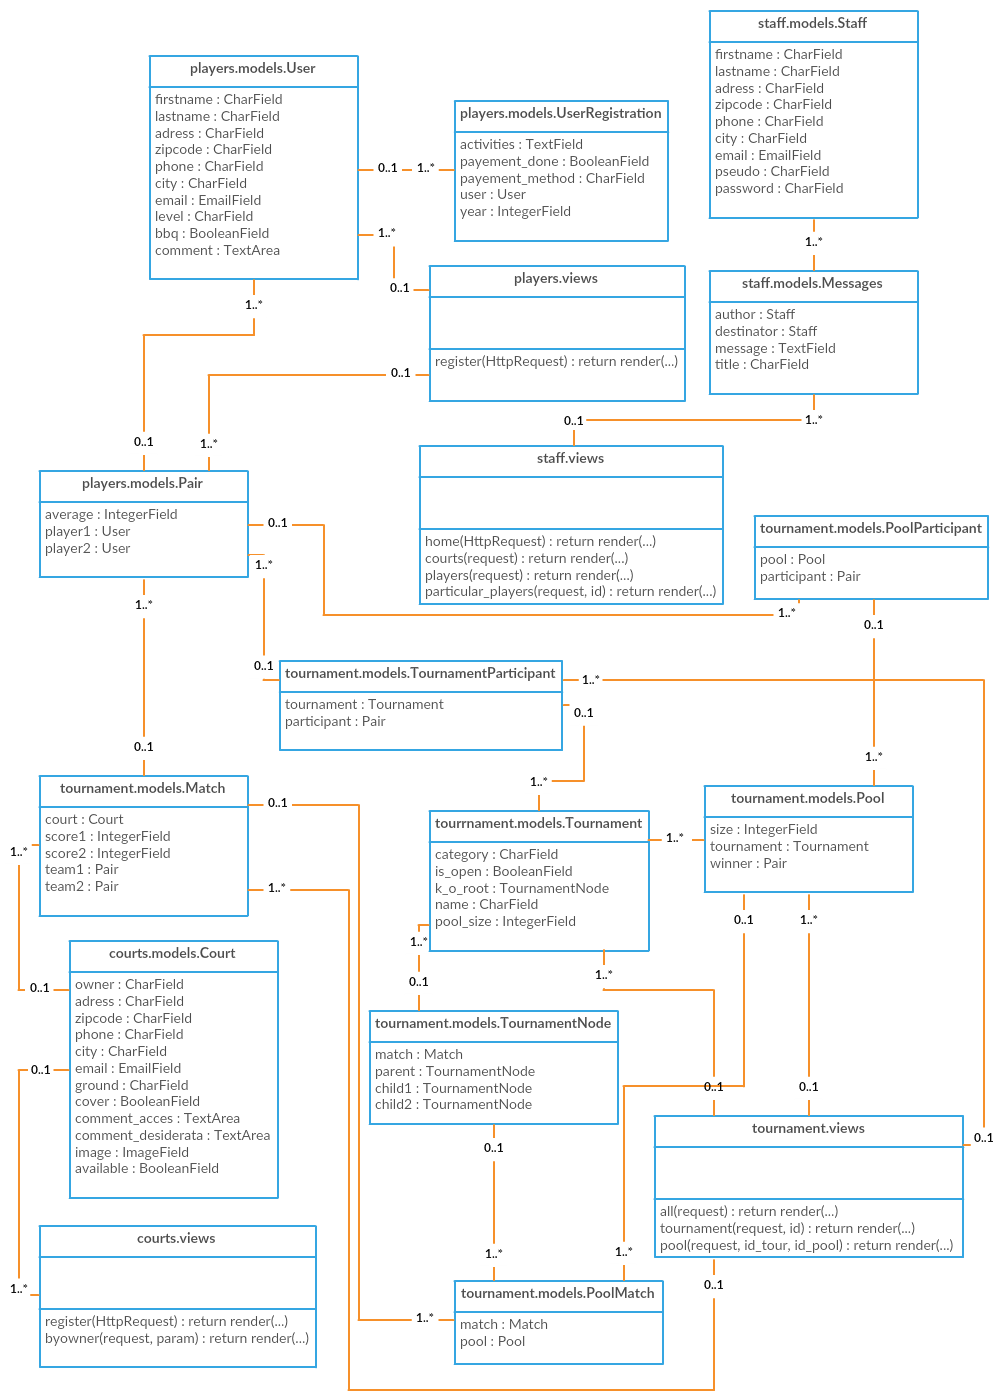
\includegraphics[scale=0.6]{UMLp2.PNG}
\end{figure}

You can see our UML diagram in Figure\ref{uml2}. The classes haven't changed since the last sprint but we modified the diagram so that it looks simpler and has less overhead.\\


Our software follows Django's architecture. We gathered all the \textit{html and css} files for the whole website. Before doing so, we had all the HTML files in the repositories of every application of the software. Now, the HTML file of each page extends the file \textit{site\_template} so that we avoid having redundancy. Moreover, this technique is more generic as well. \\
\newpage

\section{Communication with the client \& Feedback}
Days before the deadline, we contacted the clients to get some feedback on our website. We asked them to tell us what they felt were in need of a change in our software. However, they were actually not able to give us their opinion about it just yet. We will make sure to take into account the feedback received for the next sprint. \\

\section{Conclusion}
After phase 2, the website is starting to reach its final form, as more and more requirements and features start to be implemented into the website. We made sure to correct the mistakes in the ORM diagram, and correct some small details that were not working. 

\begin{appendices}
\section*{Screenshots of the website}
\noindent
\begin{figure}[b]
\caption{\label{figure2} Home page}
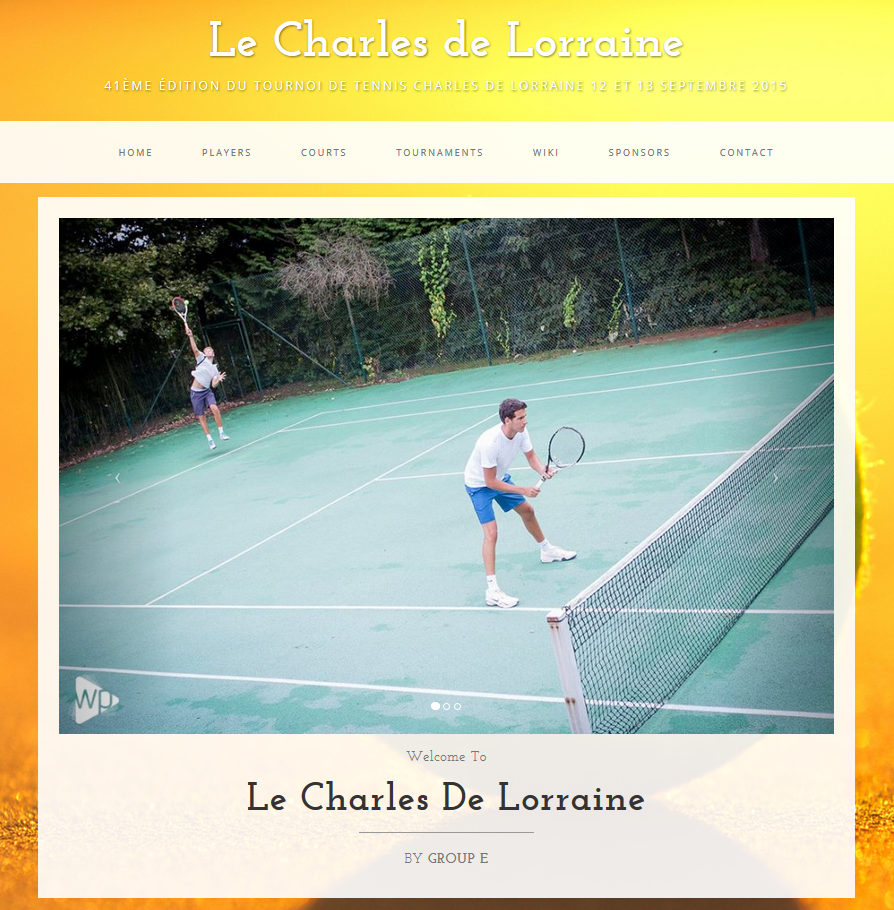
\includegraphics[scale=0.7]{site1.PNG}
\end{figure}

\begin{figure}
\caption{\label{figure3} Player(s) registration}
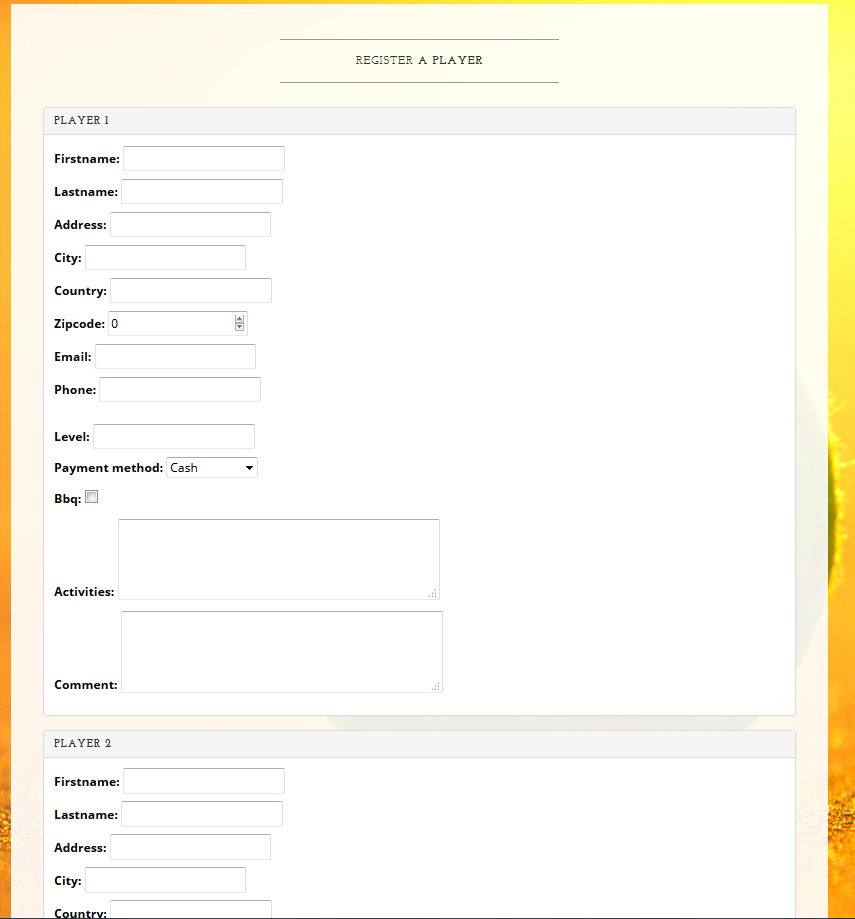
\includegraphics[scale=0.8]{site2.PNG}
\end{figure}

\begin{figure}
\caption{\label{figure4} Owner court registration}
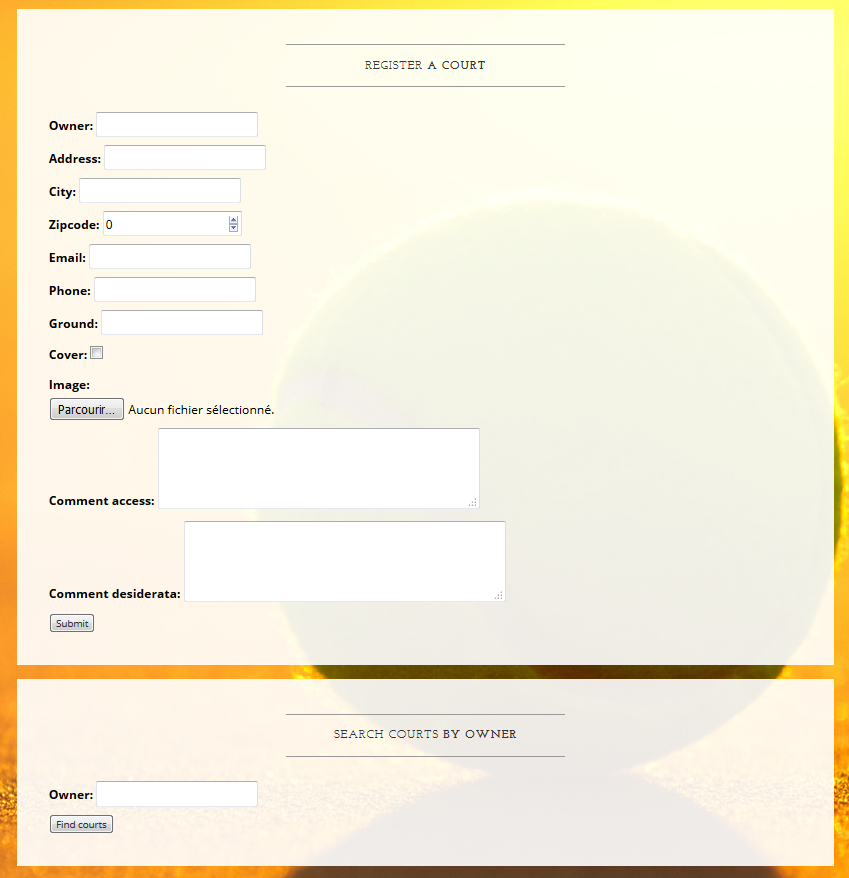
\includegraphics[scale=0.8]{site3.PNG}
\end{figure}

\begin{figure}
\caption{\label{figure5} Admin Page}
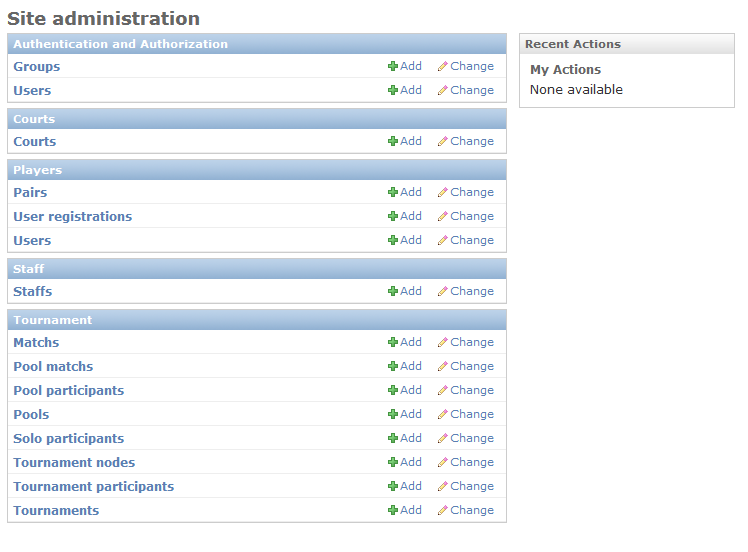
\includegraphics[scale=0.9]{site4.PNG}
\end{figure}

\begin{figure}
\caption{\label{figure6} Staff Page}
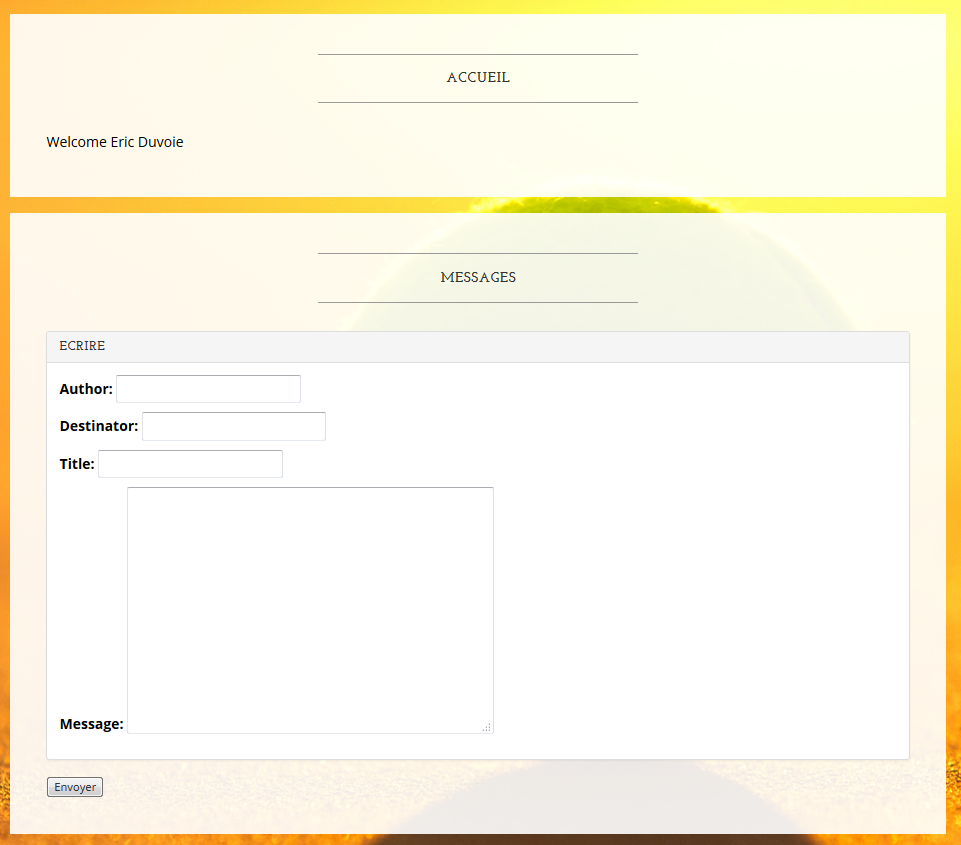
\includegraphics[scale=0.7]{site5.PNG}
\end{figure}

\end{appendices}
\end{document}